\documentclass[12pt,twoside]{article}
%%%%%%%%%%%%%%%%%%%%%%%%%%%%%%%%%%%%%%%%%%%%%%%%%%%%%%%%%%%%%
% Meta informations:
\newcommand{\trauthor}{Michael Blesel, Oliver Pola}
\newcommand{\trtype}{Seminar Paper} %{Seminararbeit} %{Proseminararbeit}
\newcommand{\trcourse}{Neural Networks}
\newcommand{\trtitle}{Boltzmann Machine}
\newcommand{\trmatrikelnummer}{6443269, 6769946}
\newcommand{\tremail}{\{3blesel, 5pola\}@informatik.uni-hamburg.de}
\newcommand{\trarbeitsbereich}{Knowledge Technology, WTM}
\newcommand{\trdate}{\today}

%%%%%%%%%%%%%%%%%%%%%%%%%%%%%%%%%%%%%%%%%%%%%%%%%%%%%%%%%%%%%
% Languages:

% Falls die Ausarbeitung in Deutsch erfolgt:
% \usepackage[german]{babel}
% \usepackage[T1]{fontenc}
% \usepackage[latin1]{inputenc}
% \usepackage[latin9]{inputenc}	 				
% \selectlanguage{german}

% If the thesis is written in English:
\usepackage[english]{babel} 						
\selectlanguage{english}

%%%%%%%%%%%%%%%%%%%%%%%%%%%%%%%%%%%%%%%%%%%%%%%%%%%%%%%%%%%%%
% Bind packages:
\usepackage{acronym}                    % Acronyms
\usepackage{algorithmic}								% Algorithms and Pseudocode
\usepackage{algorithm}									% Algorithms and Pseudocode
\usepackage{amsfonts}                   % AMS Math Packet (Fonts)
\usepackage{amsmath}                    % AMS Math Packet
\usepackage{amssymb}                    % Additional mathematical symbols
\usepackage{amsthm}
\usepackage{booktabs}                   % Nicer tables
%\usepackage[font=small,labelfont=bf]{caption} % Numbered captions for figures
\usepackage{color}                      % Enables defining of colors via \definecolor
\definecolor{uhhRed}{RGB}{254,0,0}		  % Official Uni Hamburg Red
\definecolor{uhhGrey}{RGB}{122,122,120} % Official Uni Hamburg Grey
\usepackage{fancybox}                   % Gleichungen einrahmen
\usepackage{fancyhdr}										% Packet for nicer headers
%\usepackage{fancyheadings}             % Nicer numbering of headlines

%\usepackage[outer=3.35cm]{geometry} 	  % Type area (size, margins...) !!!Release version
%\usepackage[outer=2.5cm]{geometry} 		% Type area (size, margins...) !!!Print version
%\usepackage{geometry} 									% Type area (size, margins...) !!!Proofread version
\usepackage[outer=3.15cm]{geometry} 	  % Type area (size, margins...) !!!Draft version
\geometry{a4paper,body={5.8in,9in}}

\usepackage{graphicx}                   % Inclusion of graphics
%\usepackage{latexsym}                  % Special symbols
\usepackage{longtable}									% Allow tables over several parges
\usepackage{listings}                   % Nicer source code listings
\usepackage{multicol}										% Content of a table over several columns
\usepackage{multirow}										% Content of a table over several rows
\usepackage{rotating}										% Alows to rotate text and objects
\usepackage[hang]{subfigure}            % Allows to use multiple (partial) figures in a fig
%\usepackage[font=footnotesize,labelfont=rm]{subfig}	% Pictures in a floating environment
\usepackage{tabularx}										% Tables with fixed width but variable rows
\usepackage{url,xspace,boxedminipage}   % Accurate display of URLs

\usepackage{varioref}
\usepackage[hidelinks]{hyperref}
\usepackage[capitalise,noabbrev]{cleveref}
\usepackage{todo}

\lstset{
	basicstyle=\ttfamily,
	frame=single,
	numbers=left,
	language=C,
	breaklines=true,
	breakatwhitespace=true,
	postbreak=\hbox{$\hookrightarrow$ },
	showstringspaces=false,
	upquote=true,
	tabsize=4,
	captionpos=b,
	morekeywords={int8_t,uint8_t,int16_t,uint16_t,int32_t,uint32_t,int64_t,uint64_t,size_t,ssize_t,off_t,intptr_t,uintptr_t,mode_t}
}

%%%%%%%%%%%%%%%%%%%%%%%%%%%%%%%%%%%%%%%%%%%%%%%%%%%%%%%%%%%%%
% Configurationen:

\hyphenation{whe-ther} 									% Manually use: "\-" in a word: Staats\-ver\-trag

%\lstloadlanguages{C}                   % Set the default language for listings
\DeclareGraphicsExtensions{.pdf,.svg,.jpg,.png,.eps} % first try pdf, then eps, png and jpg
\graphicspath{{./src/}} 								% Path to a folder where all pictures are located
\pagestyle{fancy} 											% Use nicer header and footer

% Redefine the environments for floating objects:
\setcounter{topnumber}{3}
\setcounter{bottomnumber}{2}
\setcounter{totalnumber}{4}
\renewcommand{\topfraction}{0.9} 			  %Standard: 0.7
\renewcommand{\bottomfraction}{0.5}		  %Standard: 0.3
\renewcommand{\textfraction}{0.1}		  	%Standard: 0.2
\renewcommand{\floatpagefraction}{0.8} 	%Standard: 0.5

% Tables with a nicer padding:
\renewcommand{\arraystretch}{1.2}

%%%%%%%%%%%%%%%%%%%%%%%%%%%%
% Additional 'theorem' and 'definition' blocks:
\theoremstyle{plain}
\newtheorem{theorem}{Theorem}[section]
%\newtheorem{theorem}{Satz}[section]		% Wenn in Deutsch geschrieben wird.
\newtheorem{axiom}{Axiom}[section] 	
%\newtheorem{axiom}{Fakt}[chapter]			% Wenn in Deutsch geschrieben wird.
%Usage:%\begin{axiom}[optional description]%Main part%\end{fakt}

\theoremstyle{definition}
\newtheorem{definition}{Definition}[section]

%Additional types of axioms:
\newtheorem{lemma}[axiom]{Lemma}
\newtheorem{observation}[axiom]{Observation}

%Additional types of definitions:
\theoremstyle{remark}
%\newtheorem{remark}[definition]{Bemerkung} % Wenn in Deutsch geschrieben wird.
\newtheorem{remark}[definition]{Remark} 

%%%%%%%%%%%%%%%%%%%%%%%%%%%%
% Provides TODOs within the margin:
\newcommand{\TODO}[1]{\marginpar{\emph{\small{{\bf TODO: } #1}}}}

%%%%%%%%%%%%%%%%%%%%%%%%%%%%
% Abbreviations and mathematical symbols
\newcommand{\modd}{\text{ mod }}
\newcommand{\RS}{\mathbb{R}}
\newcommand{\NS}{\mathbb{N}}
\newcommand{\ZS}{\mathbb{Z}}
\newcommand{\dnormal}{\mathit{N}}
\newcommand{\duniform}{\mathit{U}}

\newcommand{\erdos}{Erd\H{o}s}
\newcommand{\renyi}{-R\'{e}nyi}
%%%%%%%%%%%%%%%%%%%%%%%%%%%%%%%%%%%%%%%%%%%%%%%%%%%%%%%%%%%%%
% Document:
\begin{document}
\renewcommand{\headheight}{14.5pt}

\fancyhead{}
\fancyhead[LE]{ \slshape \trauthor}
\fancyhead[LO]{}
\fancyhead[RE]{}
\fancyhead[RO]{ \slshape \trtitle}

%%%%%%%%%%%%%%%%%%%%%%%%%%%%
% Cover Header:
\begin{titlepage}
	\begin{flushleft}
		Universit\"at Hamburg\\
		Department Informatik\\
		\trarbeitsbereich\\
	\end{flushleft}
	\vspace{3.5cm}
	\begin{center}
		\huge \trtitle\\
		OUTLINE
	\end{center}
	\vspace{3.5cm}
	\begin{center}
		\normalsize\trtype\\
		[0.2cm]
		\Large\trcourse\\
		[1.5cm]
		\Large \trauthor\\
		[0.2cm]
		\normalsize Matr.Nr. \trmatrikelnummer\\
		[0.2cm]
		\normalsize\tremail\\
		[1.5cm]
		\Large \trdate
	\end{center}
	\vfill
\end{titlepage}

	%backsite of cover sheet is empty!
\thispagestyle{empty}
\hspace{1cm}
\newpage

%%%%%%%%%%%%%%%%%%%%%%%%%%%%
% Abstract:

% Abstract gives a brief summary of the main points of a paper:
\section*{Abstract}

Here will be an abstract.


% Lists:
\setcounter{tocdepth}{2} 					% depth of the table of contents (for Seminars 2 is recommented)
\tableofcontents
\pagenumbering{arabic}
\clearpage

%%%%%%%%%%%%%%%%%%%%%%%%%%%%
% Content:

% the actual content, usually separated over a number of sections
% each section is assigned a label, in order to be able to put a
% crossreference to it

\section{Introduction}
\label{sec:intro}

The idea of a Boltzmann Machine (BM) is quite old~\cite{Ackley}. Similar to neural networks in general, the topic has been asleep for quite a while. Now that we have the necessary computing power, it's time to revive those ideas.


\section{Boltzmann Machine}
\label{sec:bm}

% Here we will give an introduction to the theoretical concept of a BM. It is based on concepts from physics, especially statistical mechanics, like the Ising model~\cite{Ising}. Idea is to have a stochastic neural network that finds a ``energy minimum'' while a overall ``temperature'' is slowly reduced.

In this chapter we will give a general explanation of the Boltzmann machine. We will go into the structure of the network, some theoretical background,
how the learning and recall phases work and talk about the differences between the asynchronous and synchronous update procedures.

The Boltzmann machine is a stochastic recurrent neural network with symmetrical connections.
It does unsupervised learning and tries to extract key features from the given training data.
\todo{general concept of the BM, probability distribution over input data}


\begin{figure}[h]
	\centering
	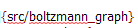
\includegraphics[height=0.2\textheight]{src/boltzmann_graph}
	\caption{Representation of a small Boltzmann machine}
    % https://upload.wikimedia.org/wikipedia/commons/thumb/7/7a/Boltzmannexamplev1.png/330px-Boltzmannexamplev1.png
	\label{fig:boltzmann-graph}
\end{figure}

In figure \cref{fig:boltzmann-graph} we can see the structure of a small Boltzmann machine. It consists of two layers of units which are called the visible and hidden layer.
All units in the Boltzmann machine are fully connected with symmetrical weights which means that value of the weight from units A to B is identical to
the weight from units B to A. All units in a Boltzman machine have a binary state of either one or zero, indicating if they are currently activated or not.
The weights can take any positive or negative real value.\newline
The Boltzmann machine uses unsupervised learning and has no clear output layer. The visible layer is used during training to hold the input data and
after learning the free running phase of the machine creates a binary vector of the states of the visible units which can be seen as the output.
The general idea behind the Boltzmann machine is to feed it with binary input vectors from the training dataset during the learning phase
in which the network learns the probability distribution of the set input units which will make it able to reproduce patterns of visible units
that will match the learned probability distribution in its recall phase. A clearer explanation of the learning and recall phases follows in the 
later sections of this chapter.


\subsection{Relation to the Boltzmann distribution}
\begin{itemize}
        \item introduce boltzmann distribution and how it is related to the BM
        \item explain concepts of Energy and temperature
        \item finding a minimum energy state
\end{itemize}

\subsection{The learning phase}
Before we get into the learning algorithm of the Boltzman machine we need to introduce the concept of 'clamped' and 'unclamped' units.
As mentioned before during the learning phase the visible units are set to the values of the binary input vectors from the training data.
This procedure is called 'clamping' the visible units, which means that during the positive phase of the learning
algorithm the states of these units will not change and they will influence the computed states for the hidden units.

\begin{figure}[h]
\begin{lstlisting}[escapeinside={(*}{*)},basicstyle=\footnotesize]
SET learning_epochs, co-occurance_epochs, temperature T
SET weight matrix W = 0
LEARNING():
  WHILE W continues to change DO:
    #Positive phase
    SET the sum co-occurance matrix S = 0
    FOR EACH training pattern x:
      SET visible units to x and CLAMP them
      SET hidden units to random binary states
      CALL UPDATE(learning_epochs)
      CALL COLLECT-STATISTICS()
    SET each (*$P^{+}_{ij}$*) equal to the average of (*$S_{ij}$*) over all training runs and patterns

    #Negative phase (free-running)
    SET states of all units to random binary values and UNCLAMP them
    CALL UPDATE(learning_epochs)
    SET the sum co-occurance matrix S = 0
    CALL COLLECT-STATISTICS()
    SET each (*$P^{-}_{ij}$*) equal to the average of (*$S_{ij}$*) over all training runs

    #Update weights
    Modify each weight (*$W_{ij}$*) by (*$\Delta W_{ij} = k(P^{+}_{ij} - P^{-}_{ij})$*), where k is a small constant

UPDATE(epochs):
  FOR 1 to number of epochs:
    FOR 1 to number of unclamped units:
      randomly select an unclamped unit i
      Calculate its energy difference: (*$ \Delta E_i = \sum_j W_{ij} x_j $*)
      #Stochastically decide the resulting state
      IF (*$ U[0,1] < \frac{1}{1+ e^{- \Delta E_i / T}} $*):
        SET (*$x_i = 1$*)
      ELSE:
        SET (*$x_i = 0$*)

COLLECT-STATISTICS():
  CALL UPDATE(co-occurance_epochs)
  FOR EACH pair of connected units:
    SET (*$S_{ij} = S_{ij} + x_i x_j$*)
\end{lstlisting}
\caption{The learning algorithm}
% http://gorayni.blogspot.com/2014/06/boltzmann-machines.html
\label{fig:learning-alg}
\end{figure}

In figure \cref{fig:learning-alg} we can see the basic learning algorithm of the Boltzmann machine in pseudo code form.
The code in the figure is a simplified version of the algorithm from \ref{} \todo{cite blogpost}
To best explain the algorithm we are going to divide it into four logical parts.
\begin{enumerate}
    \item \textbf{The setup phase:}\newline
        Before the learning algorithm can start we need to set up some parameters. Firstly the weight matrix is initialized with zeros.
        The choice of zero here instead of an initialization with random values as it is often done for other neural networks is
        necessary here since the weights need to be symmetric for all pairs of units as described in the introduction part of this chapter.
        The next thing to do is setting values for the temperature, learning and co-occurance epochs. 
        \todo{explain temperature}
        
        The learning and co-occurance epochs parameters will be explained in the description of the following phases.\newline
        From here on the algorithm can begin. The first thing we can see in line 4 is that the whole learning procedure (the next three steps) is
        supposed to be executed until the values of the weight matrix have converged and no more changes are observed.
        From a theoretical point of view this happens when the equilibrium state has been reached. \todo{explain in more detail or reference previous subsection}
        In our practitcal implementation the while loop is replaced by a for loop with an iteration counter that can be set before the learning process.
    \item \textbf{The positive phase:}\newline
        The actual learning algorithm starts with the so called positive phase. In this phase the given input patterns are learned.
        First the units of the visible layer are set to the values of the current input vector and all visible units are clamped.
        All unclamped units (in this case the units of the hidden layer) are initialized with random binary values.
        Now the actual updating of the states takes place by calling the update function as many times as the learning epochs variable has been set to.
        This is another parameter that has to be set before the start of the learning algorithm and which has to be tuned to fit the problem.\newline
        In the update function the stochastic update of the states of the unclamped units takes place. The update calculations are done
        step-by-step for randomly chosen unclamped units. This version of the update procedure is called asynchronous and we will
        compare it to another possible version called the synchronous update, where the updates do not take place in order
        but are computed all at once in section \cref{subsec:updating-procedures}.\newline
        % The following part probably needs to be way better explained
        For each chosen unit at first its energy difference is calculated with the formula $\Delta E_i = \sum_j W_{ij} x_j$. \todo{explain formula or cite explanation from previous section}
        \todo{explain stochastic activation formula and stuff...}
        

        This whole procedure is repeated for all given input patterns. The last step of the positive phase is the collect statistics function which will be explained in
        the 'updating the weights' segment.


    \item \textbf{The free-running phase:}\newline
        After the positive phase the negative or 'free-running' phase starts. This phase is different to the positive phase in the fact that
        now all units of both layers are treated as unclamped. This means that also the visible layers units states can now be updated.
        \todo{explain what this phase is for}

    \item \textbf{Updating the weights:}\newline
        \todo{explain co-occurance and how the weights are updated}
\end{enumerate}

\todo{summarize the algorithm, alternating postitive/negative phase...}


\subsection{The recall phase}
\begin{figure}[h]
\begin{lstlisting}[escapeinside={(*}{*)},basicstyle=\footnotesize]
SET the value of input units (if there are any) and clamp them
SET unclamped units to random values
SET epochs value
CALL UPDATE(epochs)
RETURN visible units

UPDATE(epochs):
  FOR 1 to number of epochs:
    FOR 1 to number of unclamped units:
      randomly select an unclamped unit i
      Calculate its energy difference: (*$ \Delta E_i = \sum_j W_{ij} x_j $*)
      #Stochastically decide the resulting state
      IF (*$ U[0,1] < \frac{1}{1+ e^{- \Delta E_i / T}} $*):
        SET (*$x_i = 1$*)
      ELSE:
        SET (*$x_i = 0$*)
\end{lstlisting}
\caption{The recall function}
% http://gorayni.blogspot.com/2014/06/boltzmann-machines.html
\label{fig:recall-alg}
\end{figure}

\subsection{Asynchronous vs. synchronous updating}
\label{subsec:updating-procedures}


\subsection{Applications of the Boltzmann machine}


\section{Related Work}
\label{sec:related}

Here we will mention the works on BM we found and got inspiration from, but also outline what we will do different (see Variants).


\section{Implementation}
\label{sec:impl}

We will try to implement the concept of a BM in a modern framework like Tensorflow or PyTorch, if that makes sense. That will be experiments, where we can't predict the results yet.


\section{Variants}
\label{sec:variants}

When we have an implementation that can do what code of others can do as well, we will try to contribute some new approaches and maybe enlarge the scope of problems a BM can be used for.


\subsection{Time series data}
\label{sec:variants:subsec:timeseries}

So far a BM was only applied to static data.


\subsection{Continuous data}
\label{sec:variants:subsec:continuous}

So far a BM was only applied to discrete data.


\section{Results}
\label{sec:results}

We will try to find a suitable problem set, where we can apply our implementation and can compare it to other, more standard, solutions. Also, if applicable, we compare different variants / implementations of our BM.


\section{Discussion}
\label{sec:discuss}

The discussion of the results may be included in the results chapter and not be worth a separate one. % TODO


\section{Limitations}
\label{sec:limits}

Since this is an implementation topic, the main limitations derive from our implementation and may be discussed in that chapter. So this might not result in a chapter on it's own. % TODO


\section{Conclusion}
\label{sec:concl}

We will conclude with our interpretation of the results and will point out where future work would be beneficial.


%%%%%%%%%%%%%%%%%%%%%%%%%%%%%%%%%%%%%%
% hier werden - zum Ende des Textes - die bibliographischen Referenzen
% eingebunden
%
% Insbesondere stehen die eigentlichen Informationen in der Datei
% ``bib.bib''
%
\newpage
\bibliographystyle{plain}
\addcontentsline{toc}{section}{Bibliography}% Add to the TOC
\bibliography{bib}

\end{document}


